\section*{Aufgaben 2 und 3}
In dieser Aufgabe sollte die Latenzzeit und die Bandbreite gemessen werden, die
beim kommunizieren zwischen mehreren Prozessen auftreten. Dafür wurde mit verschiedenen
Konfigurationen von beteiligten Prozessoren und Zahlen von Prozessen die Zeit gemessen,
die benötigt wird, um eine Nachricht variabler Länge von einem Prozess zum anderen
und zurück zu senden. Dabei wurde dieser Ablauf $1000$ mal wiederholt und die 
gemessene Zeit gemittelt. Der Quelltext dafür ist in \lref{pingpong} und die darin
aufgerufene Funktion in \lref{walltime} dargestellt.

\lstinputlisting[label=lst:pingpong,caption={pingpong.c}]{../code/02/pingpong.c}
\lstinputlisting[label=lst:walltime,caption={wall\_time.c}]{../code/02/wall_time.c}

Wenn man für alle geforderten Konfigurationen die Zeiten in Abhängigkeit von der
Nachrichtenlänge aufträgt, resultiert der in \fref{zeiten} dargestellte Plot.

\begin{figure}[htb]
  \centering
  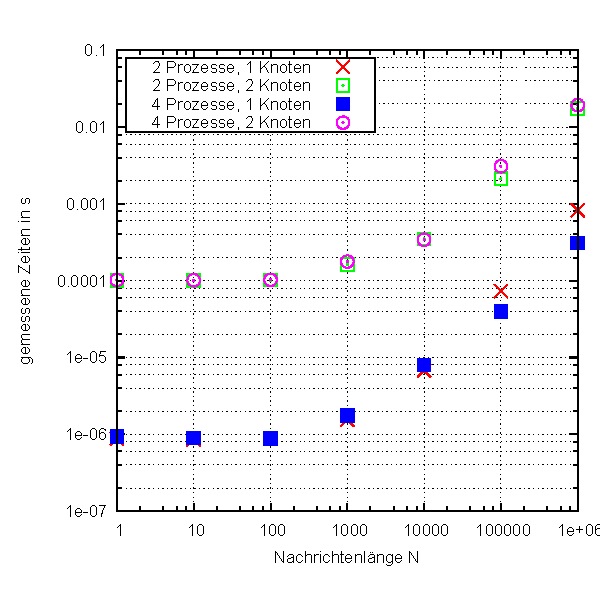
\includegraphics[width=1\columnwidth,keepaspectratio]{../tmp/zeiten}
  \caption{Gemessene Zeiten für das Senden einer Nachricht von einem Prozess zum
  anderen und zurück in Sekunden in Abhängigkeit von der Nachrichtenlänge}
  \label{fig:zeiten}
\end{figure}

